% ----------------------------------------------------------
% Teste test4_3_e25b64class10_20231212_010854
% ----------------------------------------------------------
\subsubsection{Teste test4_3_e25b64class10_20231212_010854 - AlexNet (Is That a Santa)}

Informações utilizadas para o treinamento.

\begin{table}[ht]
   \centering
   \caption{Treinamento}
   \label{tab:modelos}
   \begin{tabular}{| c | c | }
      \hline 
      \textbf{Informação} & \textbf{Descrição} \\
      \hline \hline 
      Rede & AlexNet \\
      \hline
      Número de épocas & 25\\
      \hline
      Tamanho do lote & 64\\
      \hline
      Taxa inicial & 0.012 \\
      \hline
      Taxa de decaimento & 0.0006 \\
      \hline
      Total de classes & 10\\
      \hline
      Dataset & CIFAR-10\\
      \hline
   \end{tabular} 
\end{table}

Resultados obtidos após treinamento.

\begin{tabular}{lrrrr}
\toprule
  Unnamed: 0 &  precision &  recall &  f1-score &    support \\
\midrule
    airplane &   0.836802 &  0.7640 &  0.798745 &  1000.0000 \\
  automobile &   0.910124 &  0.8810 &  0.895325 &  1000.0000 \\
        bird &   0.700000 &  0.7560 &  0.726923 &  1000.0000 \\
         cat &   0.644068 &  0.5320 &  0.582694 &  1000.0000 \\
        deer &   0.761815 &  0.8060 &  0.783285 &  1000.0000 \\
         dog &   0.651067 &  0.7930 &  0.715059 &  1000.0000 \\
        frog &   0.884009 &  0.7850 &  0.831568 &  1000.0000 \\
       horse &   0.802357 &  0.8850 &  0.841655 &  1000.0000 \\
        ship &   0.935593 &  0.8280 &  0.878515 &  1000.0000 \\
       truck &   0.847314 &  0.8990 &  0.872392 &  1000.0000 \\
    accuracy &   0.792900 &  0.7929 &  0.792900 &     0.7929 \\
   macro avg &   0.797315 &  0.7929 &  0.792616 & 10000.0000 \\
weighted avg &   0.797315 &  0.7929 &  0.792616 & 10000.0000 \\
\bottomrule
\end{tabular}


\begin{figure}[ht]
 \begin{center}
   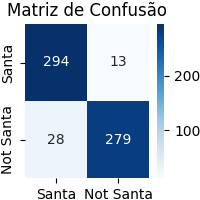
\includegraphics[scale=1]{tests/test4_3_e25b64class10_20231212_010854/confusion_matrix.png}
  \caption{Matriz de Confusão}
  \label{fig:fig03}
 \end{center}
\end{figure}

\begin{figure}[ht]
 \begin{center}
   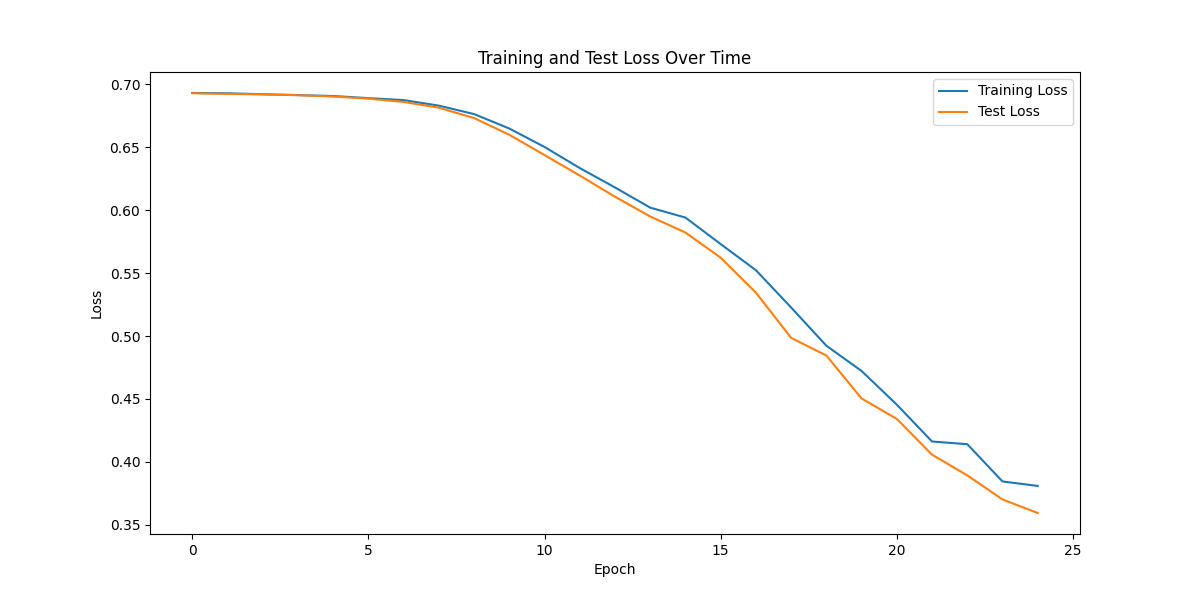
\includegraphics[scale=0.8]{tests/test4_3_e25b64class10_20231212_010854/loss_over_time.png}
  \caption{Gráfico de Perda}
  \label{fig:fig04}
 \end{center}
\end{figure}
